%
% main.tex
%
% Copyright © 2019 by Universidade Federal de Santa Catarina.
%
% OBDH 2.0 Documentation
%
% This work is licensed under the Creative Commons Attribution-ShareAlike 4.0
% International License. To view a copy of this license,
% visit http://creativecommons.org/licenses/by-sa/4.0/.
%

%
% \brief Main file.
%
% \author Gabriel Mariano Marcelino <gabriel.mm8@gmail.com>
%
% \institution Universidade Federal de Santa Catarina (UFSC)
%
% \version 0.1.0
%
% \date 18/07/2019
%

\documentclass[a4paper,12pt]{book}

\usepackage{spacelab_book}

\title{OBDH 2.0 Documentation}
\author{SpaceLab}
\date{\today}

% File metadata
\hypersetup
{
    pdfauthor   = {SpaceLab},
    pdfsubject  = {\thetitle},
    pdftitle    = {\thetitle},
    pdfkeywords = {Nanosatellites, Cubesats, OBDH}
}

\begin{document}

    \pagenumbering{roman}
    \setcounter{page}{1}

    %
% titlepage.tex
%
% Copyright (C) 2019 by Universidade Federal de Santa Catarina.
%
% OBDH 2.0 Documentation
%
% This work is licensed under the Creative Commons Attribution-ShareAlike 4.0
% International License. To view a copy of this license,
% visit http://creativecommons.org/licenses/by-sa/4.0/.
%

%
% \brief Title page.
%
% \author Gabriel Mariano Marcelino <gabriel.mm8@gmail.com>
%
% \institution Universidade Federal de Santa Catarina (UFSC)
%
% \version 0.1.0
%
% \date 18/07/2019
%

\begin{titlepage}

\thispagestyle{empty}

\begin{flushleft}
SPACELAB - OBDH 2 DOCUMENTATION - REV1
\end{flushleft}

\begin{figure}[!ht]
    \begin{flushleft}
        
\includegraphics[width=5cm]{figures/spacelab.png}
    \end{flushleft}
\end{figure}

\begin{flushleft}
\Huge{\textbf{\thetitle}}
\rule[0pt]{\textwidth}{5pt}
\end{flushleft}

\vspace{0.2cm}

\begin{flushleft}
\textit{\thetitle} \\
\textit{SpaceLab, Universidade Federal de Santa Catarina, Florianópolis - Brazil}
\end{flushleft}

\vfill
\vfill

\begin{flushright}
October 2019
\end{flushright}

\end{titlepage}

    \cleardoublepage
    %
% authorpage.tex
%
% Copyright (C) 2019 by Universidade Federal de Santa Catarina.
%
% OBDH 2.0 Documentation
%
% This work is licensed under the Creative Commons Attribution-ShareAlike 4.0
% International License. To view a copy of this license,
% visit http://creativecommons.org/licenses/by-sa/4.0/.
%

%
% \brief Author page.
%
% \author Gabriel Mariano Marcelino <gabriel.mm8@gmail.com>
%
% \institution Universidade Federal de Santa Catarina (UFSC)
%
% \version 0.1.0
%
% \date 18/07/2019
%

\thispagestyle{empty}

\begin{center}

\textbf{\thetitle}

\textit{October, 2019}

\vspace{1cm}

\textbf{Project Chief:}

Eduardo Augusto Bezerra

\vspace{1cm}

\textbf{Authors:}

Gabriel Mariano Marcelino \\

\vspace{1cm}

\textbf{Contributing Authors:}

%Author 1 \\
%Author 2 \\
%Author 3 \\

\vspace{1cm}


\textbf{Revision Control:}

\end{center}

\begin{table}[!ht]
    \begin{center}
        \begin{tabular}{cL{5cm}L{5.5cm}C{2cm}}
            \toprule[1.5pt]
            \textbf{Version} & \textbf{Author}  & \textbf{Changes}    & \textbf{Date} \\
            \midrule
            0.1     & Gabriel Mariano Marcelino & Document creation   & 10/2019    \\
                    &                           &                     &            \\
                    &                           &                     &            \\
                    &                           &                     &            \\
            \bottomrule[1.5pt]
        \end{tabular}
    \end{center}
\end{table}

\vfill

\begin{figure}[!h]
	\begin{center}
		\includegraphics[width=0.25\textwidth]{figures/by-sa.eps}
	\end{center}
\end{figure}

\textcopyright\  2019 by Universidade Federal de Santa Catarina. \thetitle. This work is licensed under the Creative Commons Attribution-ShareAlike 4.0 International License. To view a copy of this license, visit \href{http://creativecommons.org/licenses/by-sa/4.0/}{http://creativecommons.org/licenses/by-sa/4.0/}.

    \cleardoublepage

    \listoffigures
    \addcontentsline{toc}{chapter}{List of Figures}

    \listoftables
    \addcontentsline{toc}{chapter}{Lista of Tables}

    \printnomenclature
    \addcontentsline{toc}{chapter}{Nomenclature}

    \tableofcontents
    \cleardoublepage
    
    \pagenumbering{arabic}
    \setcounter{page}{1}

    %
% introduction.tex
%
% Copyright (C) 2019 by Universidade Federal de Santa Catarina.
%
% OBDH 2.0 Documentation
%
% This work is licensed under the Creative Commons Attribution-ShareAlike 4.0
% International License. To view a copy of this license,
% visit http://creativecommons.org/licenses/by-sa/4.0/.
%

%
% \brief Introduction chapter.
%
% \author Gabriel Mariano Marcelino <gabriel.mm8@gmail.com>
%
% \institution Universidade Federal de Santa Catarina (UFSC)
%
% \version 0.1.0
%
% \date 18/07/2019
%

\chapter{Introduction} \label{ch:introduction}

\begin{itemize}
    \item Main target: FloripaSat-2
    \item Improved version of the OBDH from FloripaSat-1
    \item Open source software (GPLv3 license)
    \item Open source hardware (GPLv3 license)
    \item RTOS
    \item Low power MCU
\end{itemize}

\begin{figure}[!ht]
    \begin{center}
        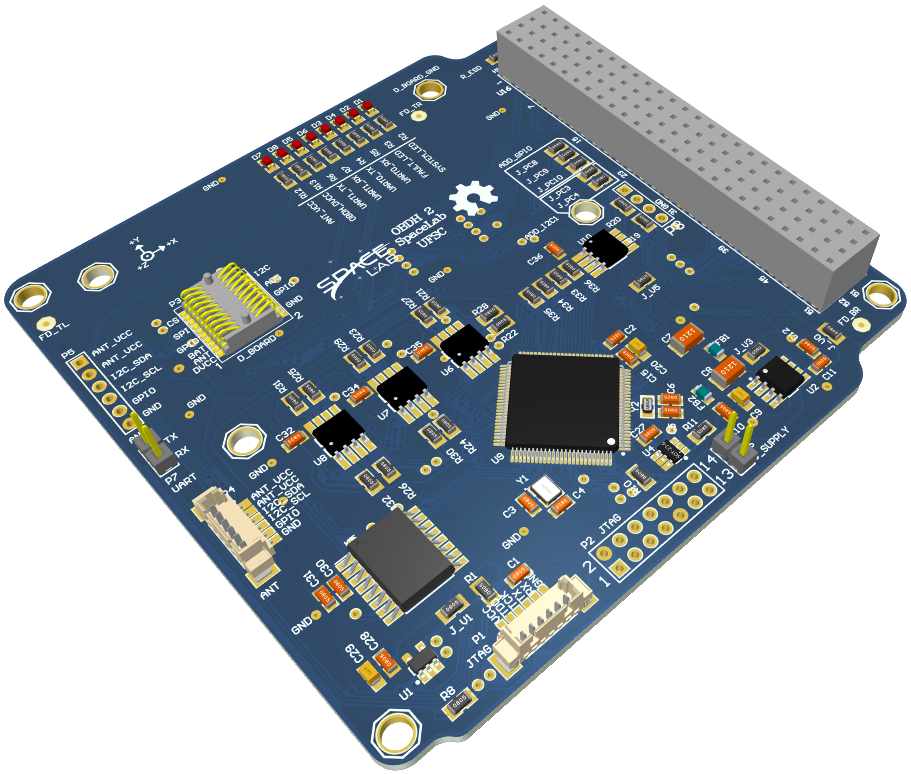
\includegraphics[width=0.75\textwidth]{figures/obdh2-pcb-3d.png}
        \caption{3D view of the OBDH 2.0 PCB.}
        \label{fig:pcb-3d}
    \end{center}
\end{figure}

    %
% requirements.tex
%
% Copyright (C) 2019 by Universidade Federal de Santa Catarina.
%
% OBDH 2.0 Documentation
%
% This work is licensed under the Creative Commons Attribution-ShareAlike 4.0
% International License. To view a copy of this license,
% visit http://creativecommons.org/licenses/by-sa/4.0/.
%

%
% \brief Requirements chapter.
%
% \author Gabriel Mariano Marcelino <gabriel.mm8@gmail.com>
%
% \institution Universidade Federal de Santa Catarina (UFSC)
%
% \version 0.1.0
%
% \date 20/10/2019
%

\chapter{Requirements} \label{ch:requirements}

    %
% system_overview.tex
%
% Copyright (C) 2019 by SpaceLab.
%
% OBDH 2.0 Documentation
%
% This work is licensed under the Creative Commons Attribution-ShareAlike 4.0
% International License. To view a copy of this license,
% visit http://creativecommons.org/licenses/by-sa/4.0/.
%

%
% \brief System Overview chapter.
%
% \author Gabriel Mariano Marcelino <gabriel.mm8@gmail.com>
%
% \institution Universidade Federal de Santa Catarina (UFSC)
%
% \version 0.1.0
%
% \date 23/11/2019
%

\chapter{System Overview} \label{ch:system-overview}

\begin{figure}[!ht]
    \begin{center}
        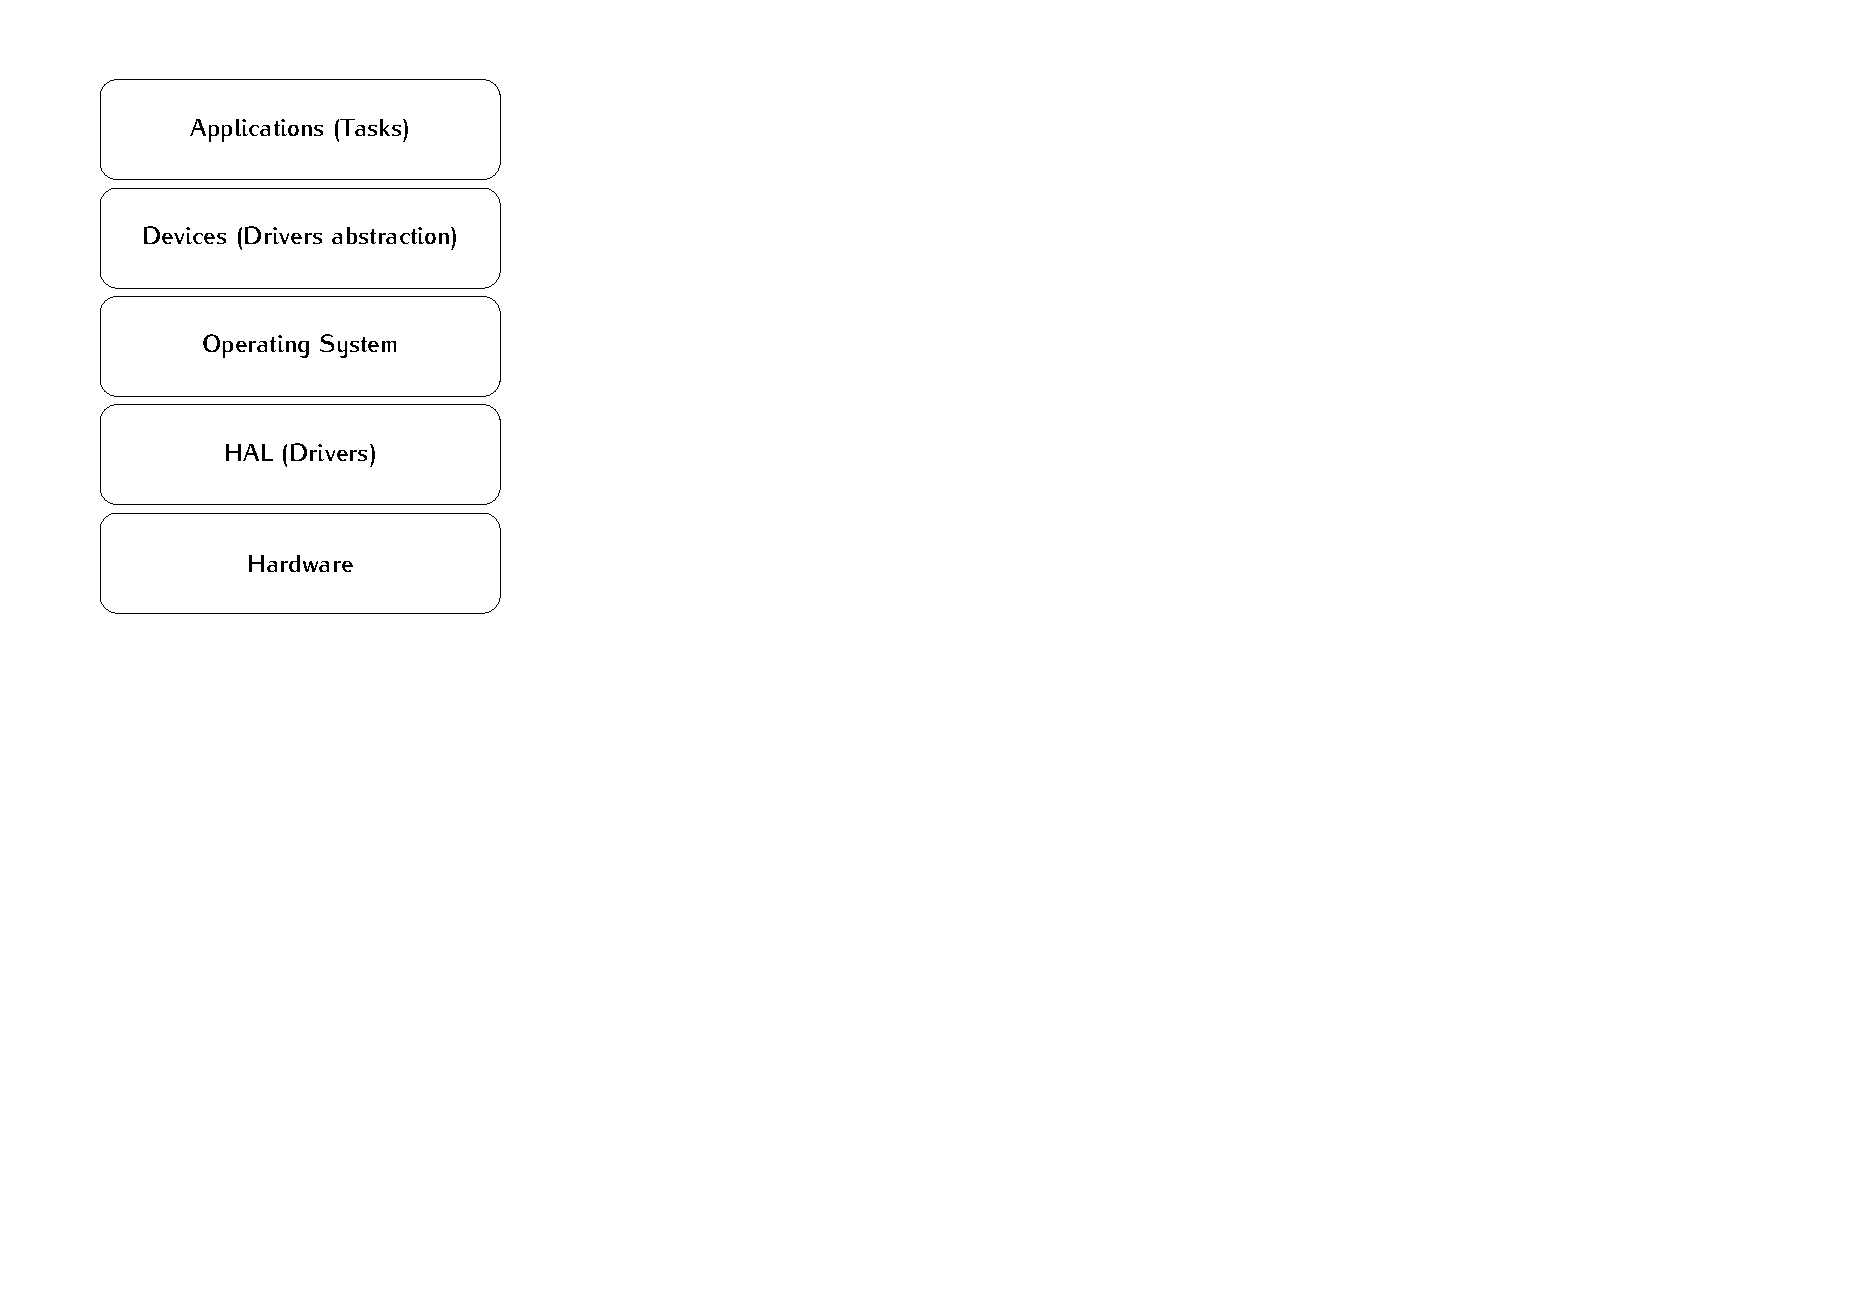
\includegraphics[width=0.4\textwidth]{figures/system_layers.pdf}
        \label{fig:system-layers}
        \caption{System layers.}
    \end{center}
\end{figure}

    %
% hardware.tex
%
% Copyright (C) 2020 by Universidade Federal de Santa Catarina.
%
% OBDH 2.0 Documentation
%
% This work is licensed under the Creative Commons Attribution-ShareAlike 4.0
% International License. To view a copy of this license,
% visit http://creativecommons.org/licenses/by-sa/4.0/.
%

%
% \brief Hardware chapter.
%
% \author Gabriel Mariano Marcelino <gabriel.mm8@gmail.com>
% \author André Martins Pio de Mattos <andrempmattos@gmail.com>
%
% \institution Universidade Federal de Santa Catarina (UFSC)
%
% \version 0.5.0
%
% \date 2019/10/20
%

\chapter{Hardware} \label{ch:hardware}

The OBDH 2.0 architecture focus on low-power operation and low-cost production, maintaining performance and proposing different approaches to increase the overall reliability. Therefore, the board was developed using these criteria and the changes from the original design were necessary to improve bottlenecks and achieve the requirements of further space mission. The \autoref{fig:block-diagram} presents the module architecture from the hardware perspective, including the main PCB components and interfaces: microcontroller, buffers, transceivers, memory, watchdog and voltage monitor, and connectors. In the following sections, the hardware design, interfaces, and standards are described in detail. The Figures \ref{fig:pcb-top}, \ref{fig:pcb-bottom} and \ref{fig:pcb-side} present 3D rendered images of the top, bottom and side views of the board, respectively.

\begin{figure}[!ht]
    \begin{center}
        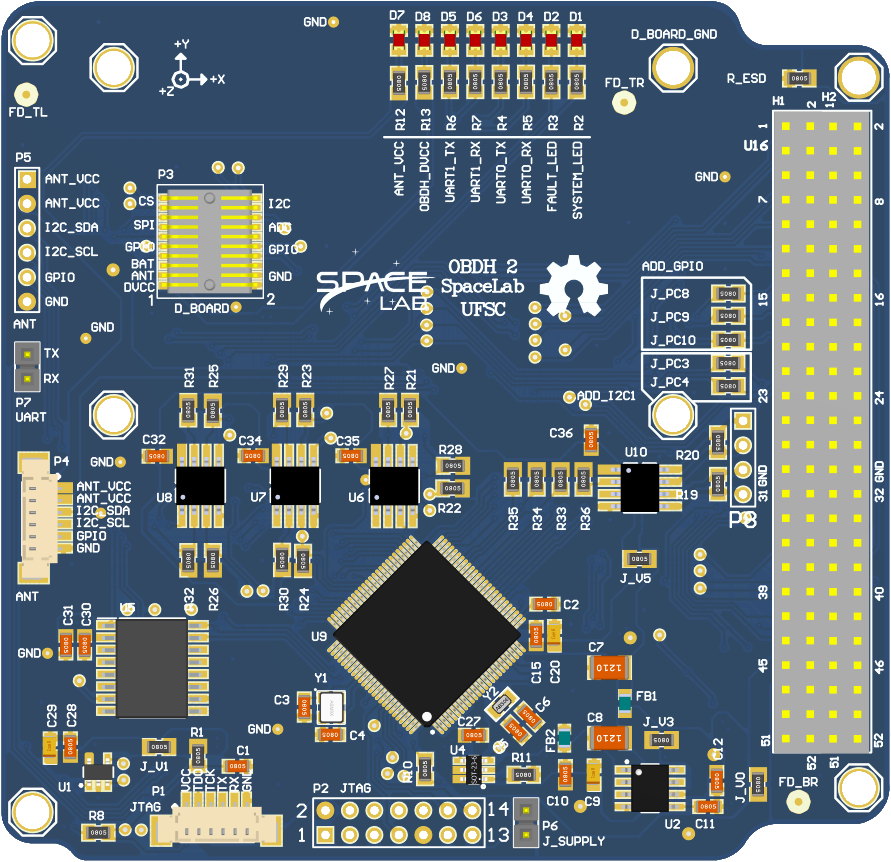
\includegraphics[width=93mm]{figures/obdh2-pcb-top.png}
        \caption{Top side of the PCB.}
        \label{fig:pcb-top}
    \end{center}
\end{figure}

\begin{figure}[!ht]
    \begin{center}
        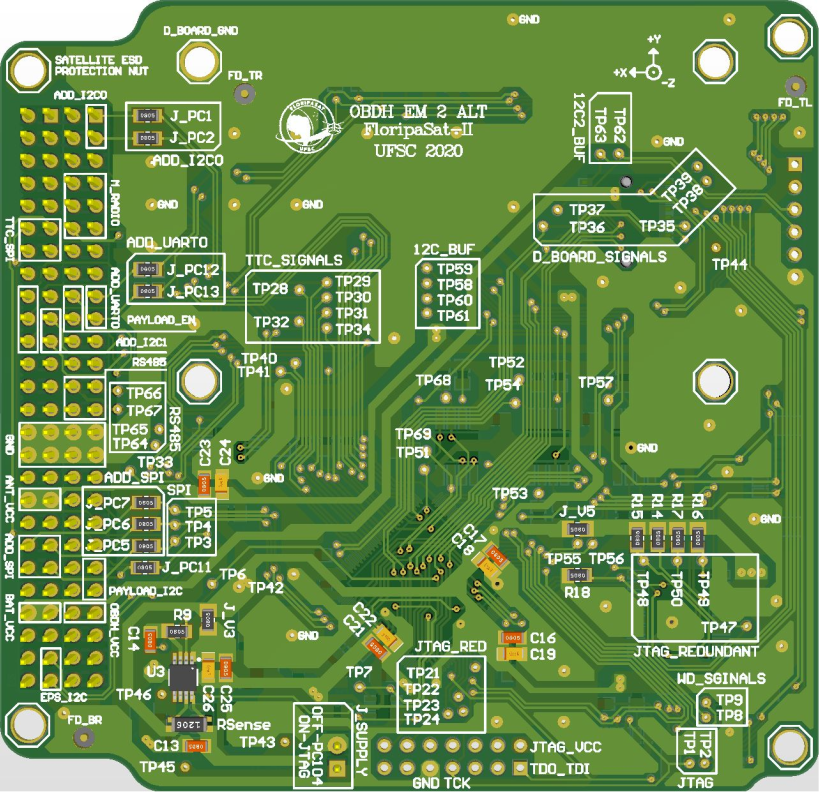
\includegraphics[width=93mm]{figures/obdh2-pcb-bottom.png}
        \caption{Bottom side of the PCB.}
        \label{fig:pcb-bottom}
    \end{center}
\end{figure}

\begin{figure}[!ht]
    \begin{center}
        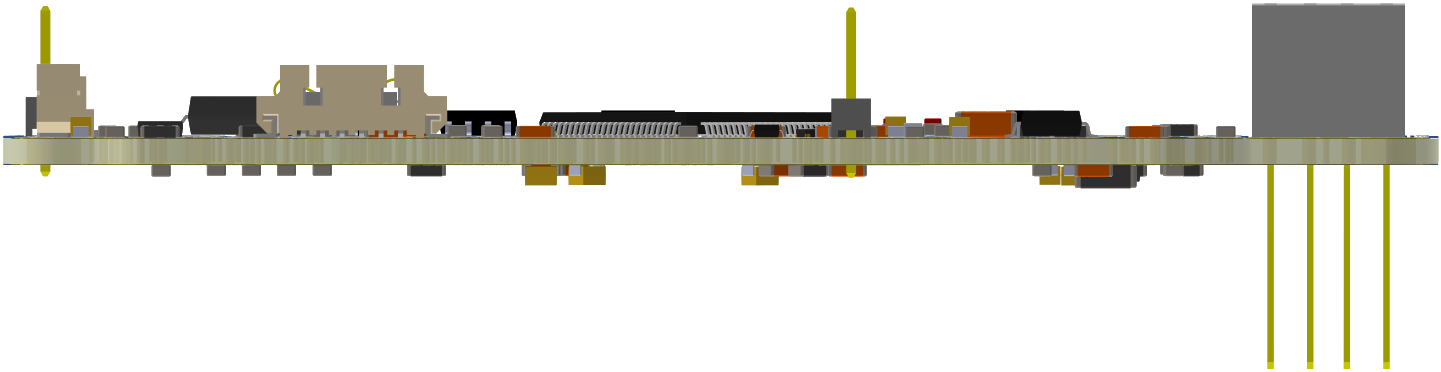
\includegraphics[width=93mm]{figures/obdh2-pcb-side.png}
        \caption{Side view of the PCB.}
        \label{fig:pcb-side}
    \end{center}
\end{figure}


\section{Interfaces}

The \autoref{fig:diagram-interfaces} presents the board interfaces, which consists of communication with other modules, debug access points, and internal peripherals. From the perspective of the microcontroller, there are 6 individual and shared communication buses and the JTAG interface, in the following scheme: A0-SPI (shared with Radio, TTC, and external memory chip); A1-UART (shared with redundant payloads); A2-UART (dedicated for debug); B0-I2C (dedicated for the payload); B1-I2C (dedicated for the EPS); B2-I2C (dedicated for the Antenna module). Currently, "\textit{Payload 1}" and "\textit{Payload 2}" are "\textit{Payload-X}" and "\textit{Payload EDC}" respectively.

\begin{figure}[!ht]
    \begin{center}
        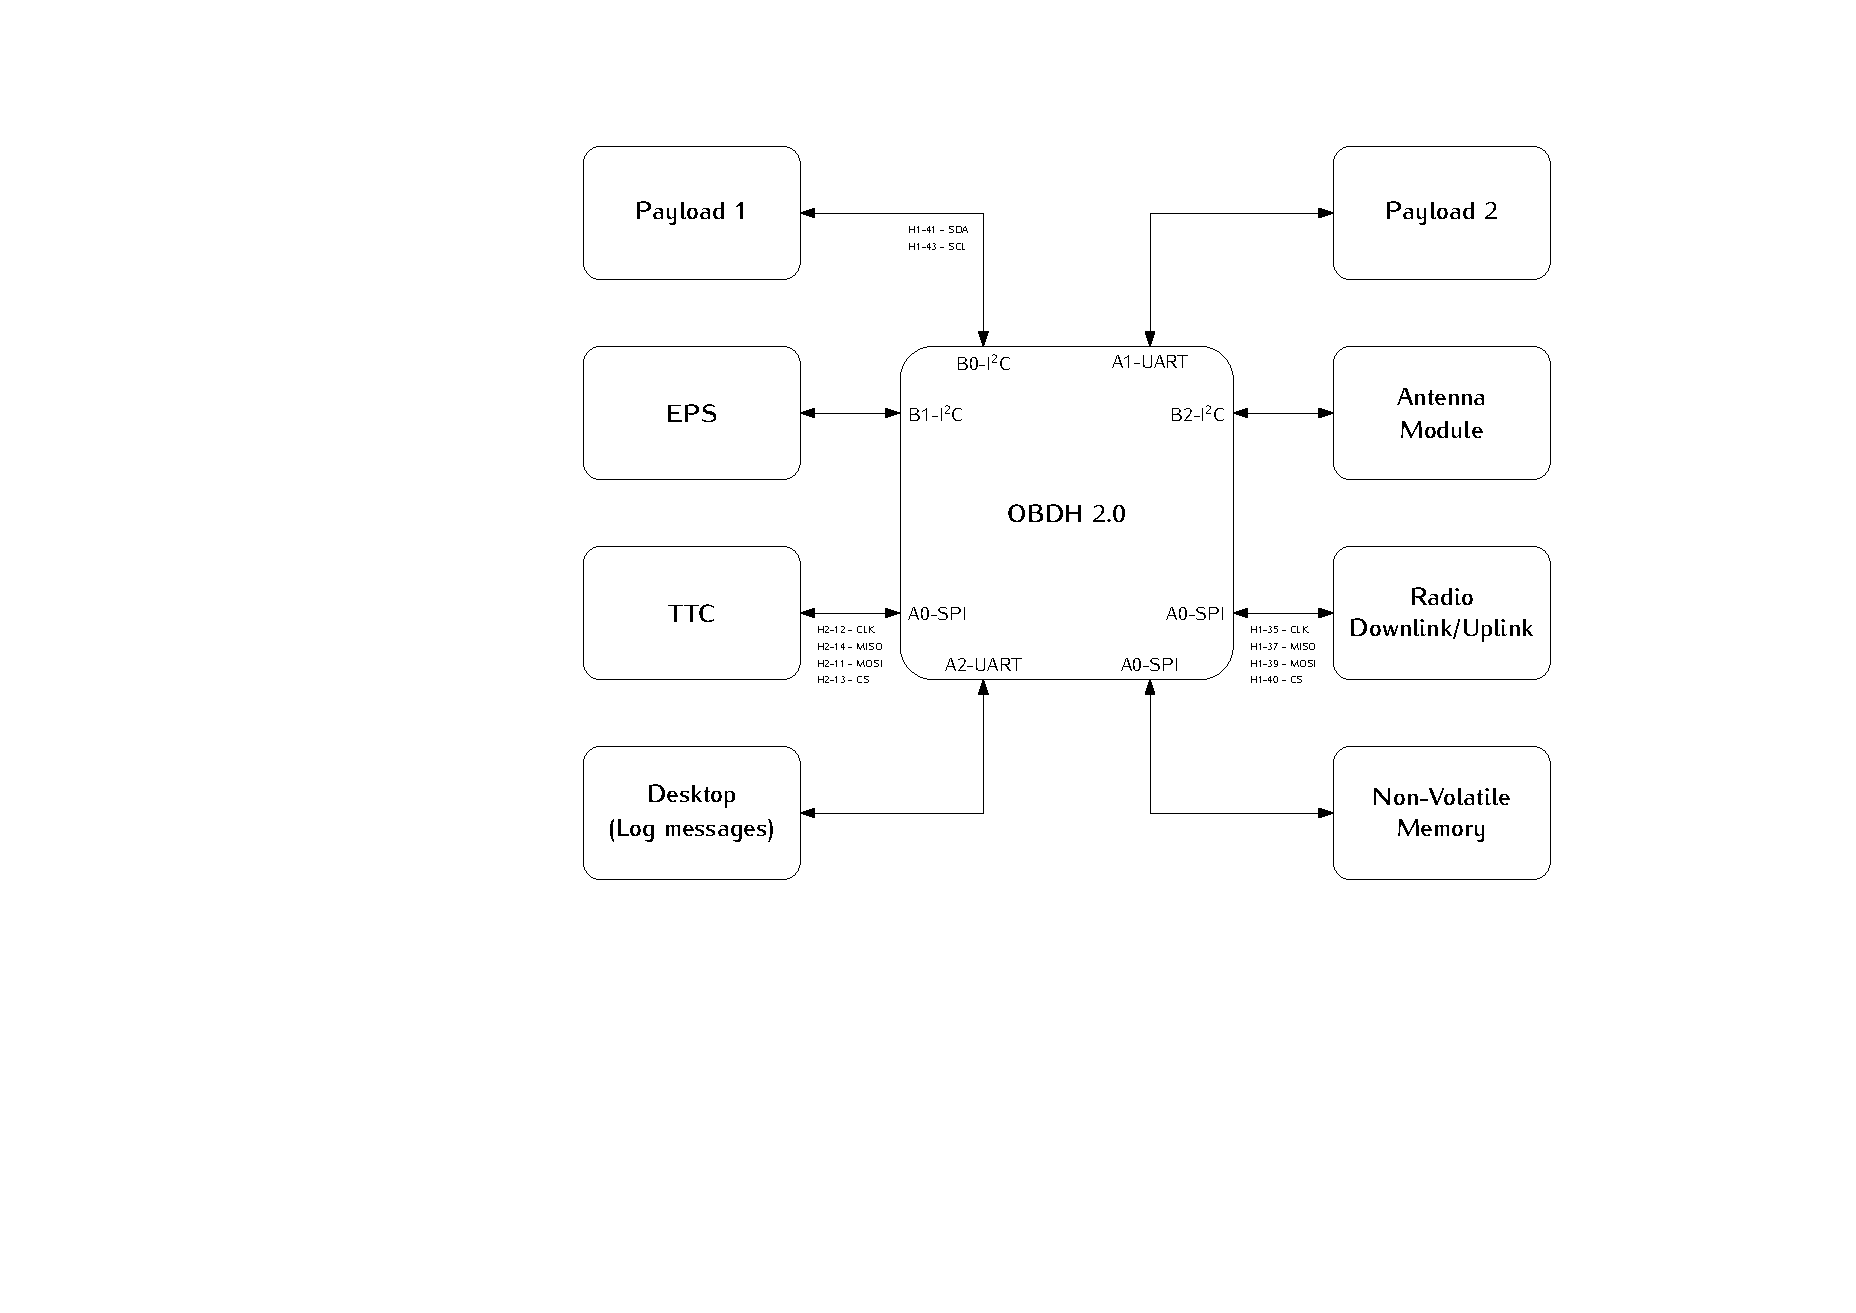
\includegraphics[width=\textwidth]{figures/diagram_interfaces.pdf}
        \caption{Interfaces diagram. \textcolor{red}{need to add jtag, daughterboard connector and update the interfaces/payload}}
        \label{fig:diagram-interfaces}
    \end{center}
\end{figure}

\section{External Connectors}

The external interfaces are connected to the microcontroller using different connector types: EPS, TTC, Radio, and Payloads through PC-104; Antenna module with 6H header and 6P picoblade connectors; JTAG through 14H header and 6P picoblade connectors; and debug access using a dedicated 2H header and shared with the JTAG connectors. The following topics describe these interfaces and present the connectors pinout.

\subsection{PC-104}

The connector referred as PC-104 is a junction of two double row 28H headers (\textit{SSW-126-04-G-D}). These connectors create a solid 104-pin interconnection across the different satellite modules. The \autoref{fig:pc-104-scheme} shows the PC-104 interface from the bottom side of the PCB, which allows visualize the simplified label scheme in the board. Also, the \autoref{tab:pc104-pins} provides the connector pinout\footnote{This pinout is simplified since additional interfaces were omitted. Refer to \textit{option sheet} in chapter \ref{ch:assembly}.} for the pins that are connected to the module. 

\begin{figure}[!ht]
    \begin{center}
        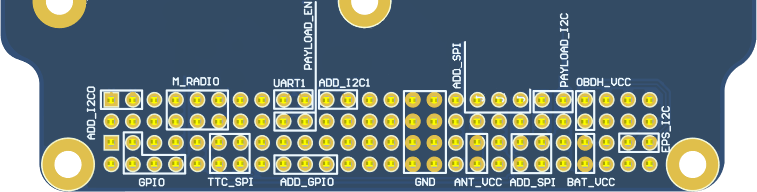
\includegraphics[width=0.75\textwidth]{figures/pc-104-scheme.png}
        \caption{Bottom view of PC-104 and simplified labels}
        \label{fig:pc-104-scheme}
    \end{center}
\end{figure}

\begin{table}[!h]
    \centering
    \begin{tabular}{cllll}
        \toprule[1.5pt]
        \textit{Pin [A-B]} & \textit{H1A}     & \textit{H1B}     & \textit{H2A}  & \textit{H2B}  \\
        \midrule
        1-2                & -                & -                & -             & -             \\
        3-4                & -                & -                & GPIO\_4       & GPIO\_5       \\
        5-6                & -                & -                & -             & -             \\
        7-8                & GPIO\_0          & GPIO\_1          & -             & GPIO\_6       \\
        9-10               & GPIO\_2          & -                & -             & -             \\
        11-12              & GPIO\_3          & GPIO\_7          & SPI\_0\_MOSI  & SPI\_0\_CLK   \\
        13-14              & -                & -                & SPI\_0\_CS\_1 & SPI\_0\_MISO  \\
        15-16              & -                & -                & -             & -             \\
        17-18              & UART\_1\_RX      & GPIO\_8          & -             & -             \\
        19-20              & UART\_1\_TX      & GPIO\_9          & -             & -             \\
        21-22              & -                & -                & -             & -             \\
        23-24              & -                & -                & -             & -             \\
        25-26              & -                & -                & -             & -             \\
        27-28              & -                & -                & -             & -             \\
        29-30              & GND              & GND              & GND           & GND           \\
        31-32              & GND              & GND              & GND           & GND           \\
        33-34              & -                & -                & -             & -             \\
        35-36              & SPI\_0\_CLK      & -                & VCC\_3V3\_ANT & VCC\_3V3\_ANT \\
        37-38              & SPI\_0\_MISO     & -                & -             & -             \\
        39-40              & SPI\_0\_MOSI     & SPI\_0\_CS\_0    & -             & -             \\
        41-42              & I2C\_0\_SDA      & -                & -             & -             \\
        43-44              & I2C\_0\_SCL      & -                & -             & -             \\
        45-46              & VCC\_3V3         & VCC\_3V3         & VCC\_BAT      & VCC\_BAT      \\
        47-48              & -                & -                & -             & -             \\
        49-50              & -                & -                & I2C\_1\_SDA   & -             \\
        51-52              & -                & -                & I2C\_1\_SCL   & -             \\
        \bottomrule[1.5pt]
    \end{tabular}
    \caption{PC-104 connector pinout. \textcolor{red}{Synchronize nomenclature}}
    \label{tab:pc104-pins}
\end{table}

\subsection{Antenna Module}

The communication with the Antenna module is performed through external connectors, which are presented in the \autoref{fig:ant-connectors}. Both connectors have the same connections, but the \ref{fig:ant-debug-connector} (6H header) is used for development and the \ref{fig:ant-main-connector} (6P picoblade) as the connector for the flight model. This interface consists of a dedicated I2C, power supply, and GPIO, which are described in the \autoref{tab:antenna-connector-pins}.

\begin{table}[!h]
    \centering
    \begin{tabular}{cllll}
        \toprule[1.5pt]
        \textit{Pin} & \textit{Row} \\
        \midrule
        1            & VCC\_3V3\_ANT  \\
        2            & VCC\_3V3\_ANT  \\
        3            & I2C\_SDA       \\
        4            & I2C\_SCL       \\
        5            & GPIO           \\
        6            & GND            \\
        \bottomrule[1.5pt]
    \end{tabular}
    \caption{Antenna module connectors pinout.}
    \label{tab:antenna-connector-pins}
\end{table}

\begin{figure}[!htb]
    \begin{center}
        \subfigure[Debug interface of the antenna module.\label{fig:ant-debug-connector}]{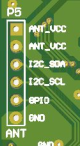
\includegraphics[width=0.135\textwidth]{figures/p5-connector.png}}
        \qquad
        \subfigure[Main interface of the antenna module.\label{fig:ant-main-connector}]{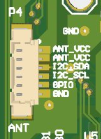
\includegraphics[width=0.205\textwidth]{figures/p4-connector.png}}
        \caption{Antenna module conectors.}
        \label{fig:ant-connectors}
    \end{center}
\end{figure}

\subsection{Programmer and Debug}

The interface with the microcontroller programmer is performed through external connectors, which are presented in the \autoref{fig:jtag-connectors}. Both connectors have the same JTAG and UART interfaces, but the 14H header is used during development and the 6P picoblade (provide more compact and reliable attachment) as the connector for the flight model, which are described in the \autoref{tab:jtag-header-connector-pins} and \autoref{tab:jtag-picoblade-connector-pins}, respectively. This interface consists of a dedicated debug UART, a JTAG, and an external power supply. The debug UART connection has another access point in a dedicated 2H header (P7), as shown in \autoref{fig:uart-debug-connector}. Also, to use this external supply, it is necessary to connect both pins of a 2H header jumper (P6).

\begin{figure}[!ht]
    \begin{center}
        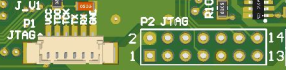
\includegraphics[width=0.7\textwidth]{figures/jtag-connector.png}
        \caption{Programmer (P1 and P2) and jumper (P6) connectors.}
        \label{fig:jtag-connectors}
    \end{center}
\end{figure}

\begin{table}[!h]
    \centering
    \begin{tabular}{cllll}
        \toprule[1.5pt]
        \textit{Pin [A-B]} & \textit{Row A} & \textit{Row B} \\
        \midrule
        1-2                & TDO\_TDI       & VCC\_3V3       \\
        3-4                & -              & -              \\
        5-6                & -              & -              \\
        7-8                & TCK            & -              \\
        9-10               & GND            & -              \\
        11-12              & -              & UART\_TX       \\
        13-14              & -              & UART\_RX       \\
        \bottomrule[1.5pt]
    \end{tabular}
    \caption{Programmer header connector pinout.}
    \label{tab:jtag-header-connector-pins}
\end{table}

\begin{table}[!h]
    \centering
    \begin{tabular}{cllll}
        \toprule[1.5pt]
        \textit{Pin} & \textit{Row} \\
        \midrule
        1            & VCC\_3V3       \\
        2            & TDO\_TDI       \\
        3            & TCK            \\
        4            & UART\_TX       \\
        5            & UART\_RX       \\
        6            & GND            \\
        \bottomrule[1.5pt]
    \end{tabular}
    \caption{Programmer picoblade connector pinout.}
    \label{tab:jtag-picoblade-connector-pins}
\end{table}

\begin{figure}[!ht]
    \begin{center}
        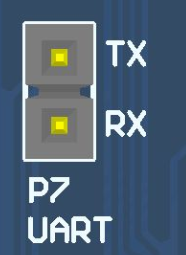
\includegraphics[width=0.15\textwidth]{figures/p7-connector.png}
        \caption{Dedicated UART debug connectors (P7).}
        \label{fig:uart-debug-connector}
    \end{center}
\end{figure}

\subsection{Daughterboard}

The daughterboard interface uses the Samtec FSI-110-D connector \cite{fsi-conn}, which can be seen in the \autoref{fig:samtec-connector}. This connector has metal contacts in format of arcs that are flexible and four polymer guide pins (a pair for top and bottom). When the daughterboard is attached, there is some pressure to this metal contacts that bend and create a meaningful pin connection to the daughterboard copper pads\footnote{These daughterboard pads are similar to the ones used as footprint in the OBDH, despite a slightly bigger size.}. A picture of this connector on the PCB can be seen in \autoref{fig:daughterboard-connector}.

\begin{figure}[!ht]
    \begin{center}
        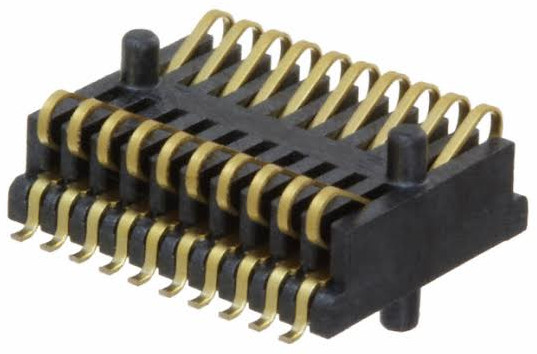
\includegraphics[width=0.4\textwidth]{figures/samtec_fsi-110-03-g-d-ad.jpeg}
        \caption{Samtec FSI-110-03-G-D-AD connector.}
        \label{fig:samtec-connector}
    \end{center}
\end{figure}

\begin{figure}[!ht]
    \begin{center}
        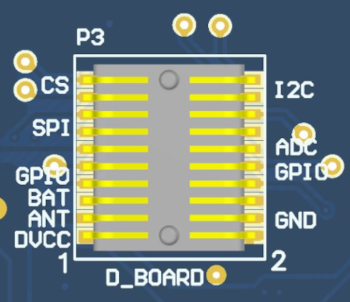
\includegraphics[width=0.3\textwidth]{figures/p3-connector.png}
        \caption{Daughterboard connector (P3).}
        \label{fig:daughterboard-connector}
    \end{center}
\end{figure}

The pinout of the daughterboard interface are available in the \autoref{tab:daugtherboard-connector-pins}. There are different power supply lines (OBDH, Antenna, and battery), communication buses (I2C and SPI), GPIO, and ADC interfaces available. Besides the GPIO and ADC pins, the other interfaces are shared with other modules and peripherals.

\begin{table}[!h]
    \centering
    \begin{tabular}{cllll}
        \toprule[1.5pt]
        \textit{Pin [A-B]} & \textit{Row A} & \textit{Row B} \\
        \midrule
        1-2                & VCC\_3V3       & GND            \\
        3-4                & VCC\_3V3\_ANT  & GND            \\
        5-6                & VCC\_BAT       & GND            \\
        7-8                & GPIO\_0        & GPIO\_1        \\
        9-10               & GPIO\_2        & GPIO\_3        \\
        11-12              & SPI\_0\_CLK    & ADC\_0         \\
        13-14              & SPI\_0\_MISO   & ADC\_1         \\
        15-16              & SPI\_0\_MOSI   & ADC\_2         \\
        17-18              & SPI\_0\_CS\_0  & I2C\_2\_SDA    \\
        19-20              & SPI\_0\_CS\_1  & I2C\_2\_SCL    \\
        \bottomrule[1.5pt]
    \end{tabular}
    \caption{Daughterboard connector pinout.}
    \label{tab:daugtherboard-connector-pins}
\end{table}

\subsubsection{Guidelines}

The recommended shape and size of the daughterboard can be seen in the \autoref{fig:daughterboard-size}. Besides that, there are mandatory and suggested elements placement: four M3 holes for mechanical attachment, required; contact connector pads (in light gray on the bottom layer), required; two debug headers in the left and bottom sides, suggested; and a general purpose flight model picoblade, suggested.

\begin{figure}[!ht]
    \begin{center}
        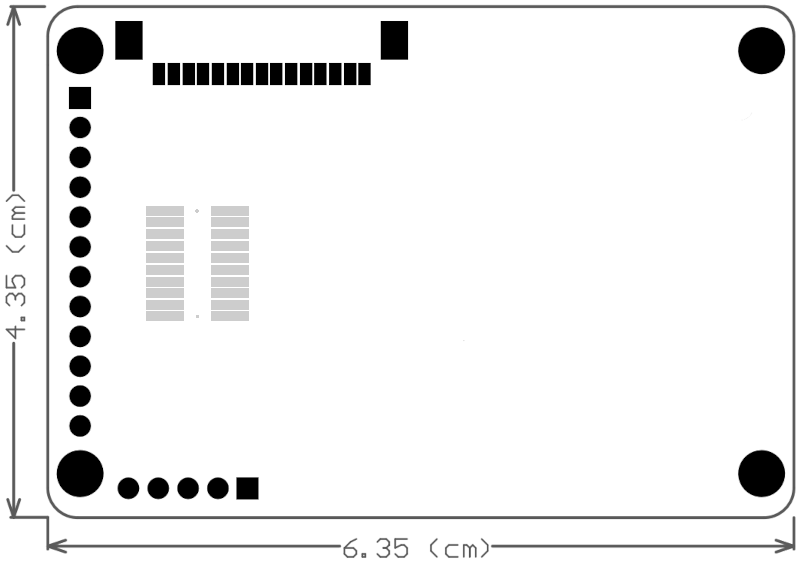
\includegraphics[width=0.52\textwidth]{figures/daughterboard-size.png}
        \caption{Recommended shape and size of the daughterboard.}
        \label{fig:daughterboard-size}
    \end{center}
\end{figure}

\begin{figure}[!ht]
    \begin{center}
        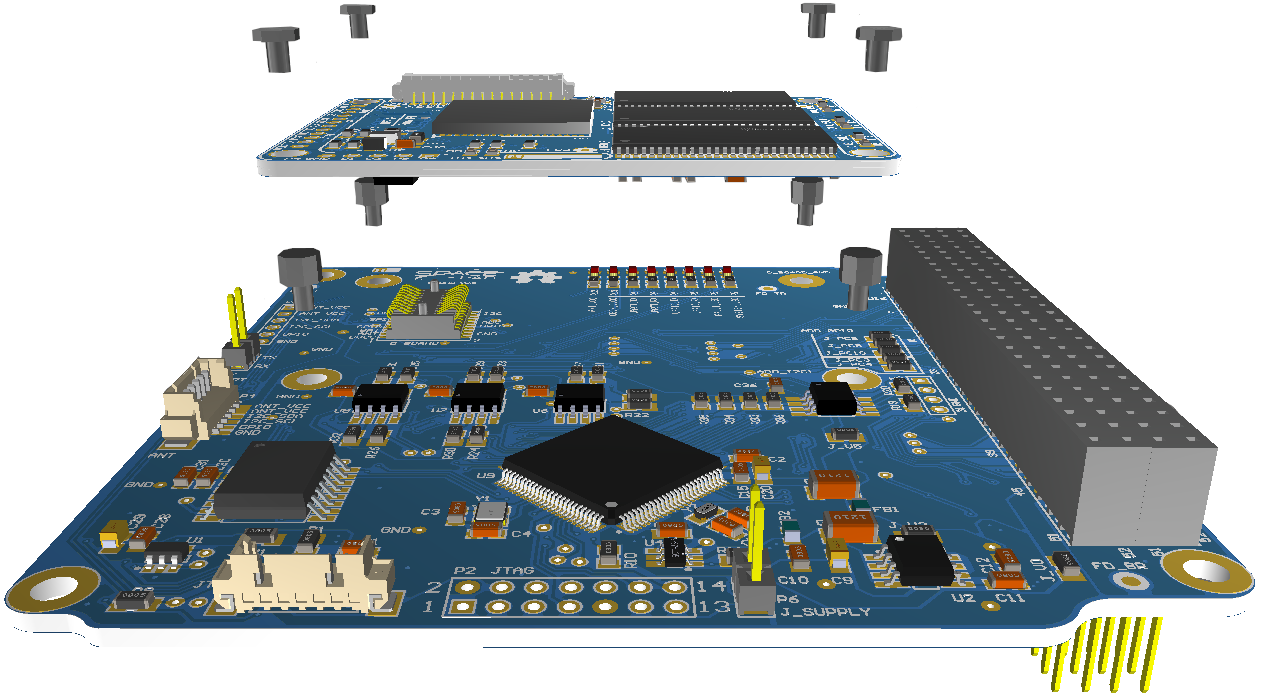
\includegraphics[width=0.6\textwidth]{figures/daughterboard-integration.png}
        \caption{Illustrative daughterboard integration.}
        \label{fig:daughterboard-integration}
    \end{center}
\end{figure}

\section{Microcontroller}

The OBDH 2.0 uses a low-power and low-cost microcontroller family from Texas Instruments, the MSP430F6659 \cite{msp430f6659}. This device provide sufficient performance for low and medium complexity software and algorithms, allowing the module to execute the required tasks. The \autoref{tab:msp430-summary} presents a summary of the main available features and \autoref{fig:msp430-diagram} shows the internal subsystems, descriptions, and peripherals. The microcontroller interfaces, configurations, and auxiliary components are described in the following topics.

\begin{table}[!h]
    \centering
    \begin{tabular}{cllllllll}
        \toprule[1.5pt]
        \textit{Flash} & \textit{SRAM} & \textit{Timers} & \textit{USCI} & \textit{ADC} & \textit{DAC} & \textit{GPIO} \\
        \midrule
        512KB  & 64KB  & 2  & 6 (SPI / I2C / UART)  & 12  & 2  & 74           \\
        \bottomrule[1.5pt]
    \end{tabular}
    \caption{Microcontroller features summary.}
    \label{tab:msp430-summary}
\end{table}

\begin{figure}[!ht]
    \begin{center}
        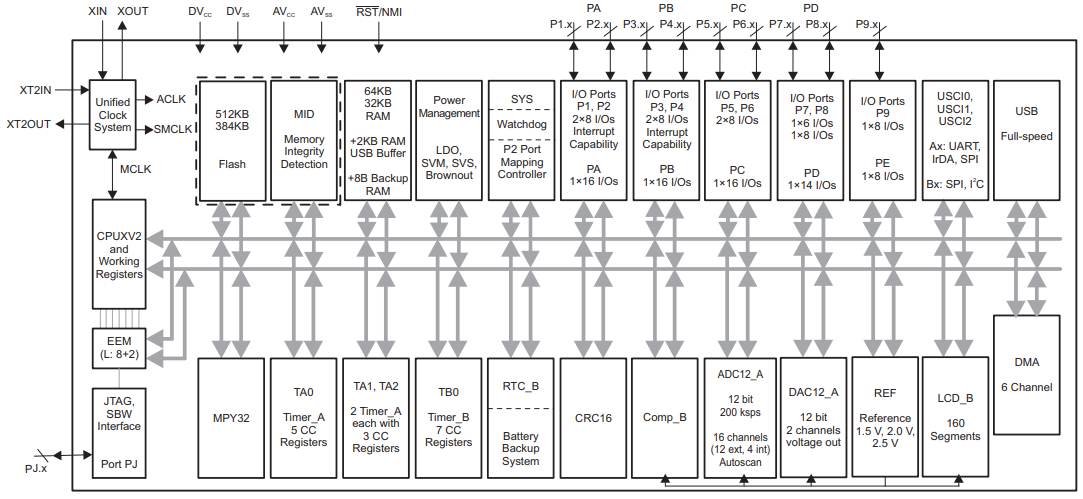
\includegraphics[width=\textwidth]{figures/msp430-diagram.png}
        \caption{Microcontroller internal diagram.}
        \label{fig:msp430-diagram}
    \end{center}
\end{figure}

\subsection{Interfaces Configuration}

The microcontroller has 6 Universal Serial Communication Interfaces (USCI) that can be configured to operate with different protocols and parameters. These interfaces are connected to different modules and peripherals, as presented in the \autoref{fig:diagram-interfaces}. The \autoref{tab:usci-config} describes each interface configurations.

\begin{table}[!h]
    \centering
    \begin{tabular}{lrrrrl}
        \toprule[1.5pt]
        \textit{Interface} & \textit{Protocol (Index)} & \textit{Mode} & \textit{Word Length} & \textit{Data Rate} & \textit{Configuration} \\
        \midrule
        USCI\_A0           & SPI                       & Master        & 8 bits               & 400 kbps           & Phase: High \\
                           &                           &               &                      &                    & Polarity: Low \\
        USCI\_A1           & UART1                     & -             & 8 bits               & 115200 bps         & Stop bits: 1 \\
                           &                           &               &                      &                    & Parity: None \\
        USCI\_A2           & UART0                     & -             & 8 bits               & 115200 bps         & Stop bits: 1 \\
                           &                           &               &                      &                    & Parity: None \\
        USCI\_B0           & I2C0                      & Master        & 8 bits               & 100 kbps           & Adr. len: 7 bits \\
        USCI\_B1           & I2C1                      & Master        & 8 bits               & 100 kbps           & Adr. len: 7 bits \\
        USCI\_B2           & I2C2                      & Master        & 8 bits               & 100 kbps           & Adr. len: 7 bits \\
        \bottomrule[1.5pt]
    \end{tabular}
    \caption{USCI configuration.}
    \label{tab:usci-config}
\end{table}

\subsection{Clocks Configuration}

Besides the internal clock sources, the microcontroller has two dedicated clock inputs for external crystals: the main clock and the auxiliary clock inputs. There are a 32MHz crystal and a 32.769kHz connected to these inputs, respectively. The first source is used for generating the Master Clock (MCLK) and the Subsystem Master Clock (SMCLK), which are used by the CPU and the internal peripheral modules. The second source is used for generating the Auxiliary Clock (ACLK) that handles the low-power modes and might be used for peripherals.

\subsection{Pinout}

An illustration of the microcontroller pinout positions can be seen in the \autoref{fig:msp430-pinout-positions}. The \autoref{tab:mcu-pinout} presents the OBDH 2.0 microcontroller pins assignment.

\begin{figure}[!ht]
    \begin{center}
        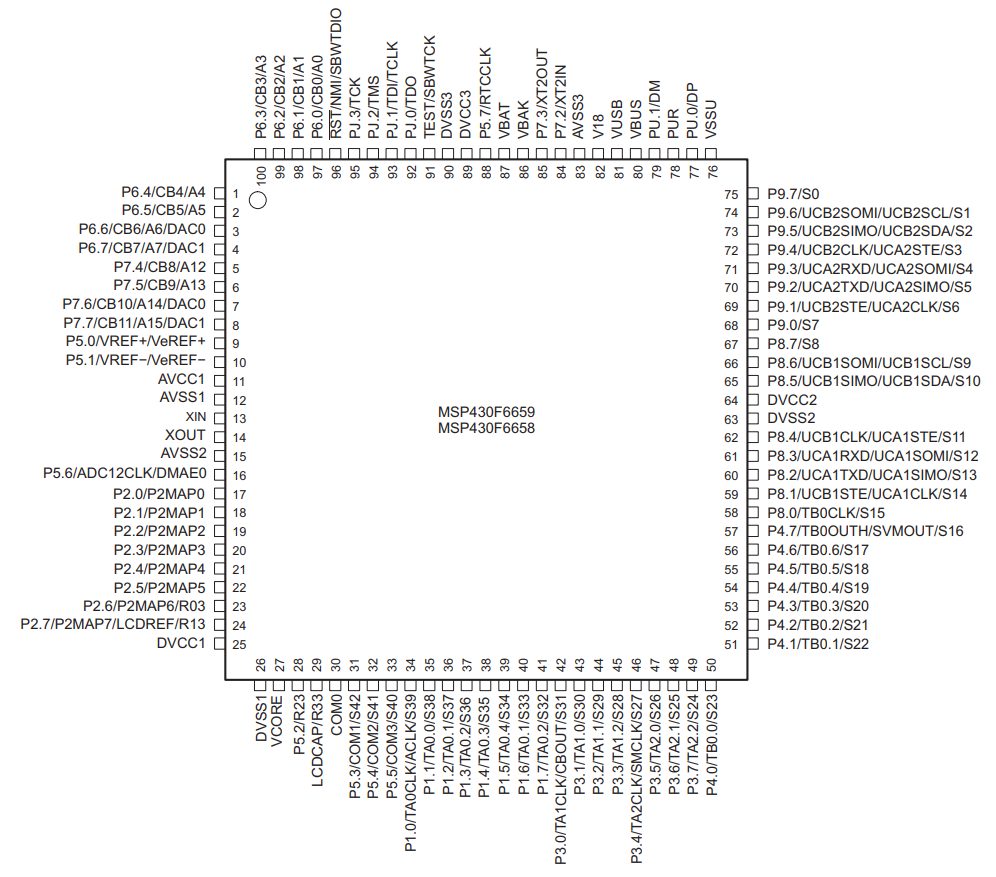
\includegraphics[width=0.9\textwidth]{figures/msp430-pinout.png}
        \caption{Microcontroller pinout positions.}
        \label{fig:msp430-pinout-positions}
    \end{center}
\end{figure}

\begin{longtable}{lcl}
    \toprule[1.5pt]
    \textit{Pin Code} & \textit{Pin Number} & \textit{Signal}       \\
    \midrule
    P1.0              & 34                  & MAIN\_RADIO\_ENABLE   \\
    P1.1              & 35                  & MAIN\_RADIO\_GPIO0    \\
    P1.2              & 36                  & MAIN\_RADIO\_GPIO1    \\
    P1.3              & 37                  & MAIN\_RADIO\_GPIO2    \\
    P1.4              & 38                  & MAIN\_RADIO\_RESET    \\
    P1.5              & 39                  & MAIN\_RADIO\_SPI\_CS  \\
    P1.6              & 40                  & TTC\_MCU\_SPI\_CS     \\
    P1.7              & 41                  & -                     \\
    \midrule
    P2.0              & 17                  & SPI\_CLK              \\
    P2.1              & 18                  & I2C0\_SDA             \\
    P2.2              & 19                  & I2C0\_SCL             \\
    P2.3              & 20                  & -                     \\
    P2.4              & 21                  & SPI\_MOSI             \\
    P2.5              & 22                  & SPI\_MISO             \\
    P2.6              & 23                  & -                     \\
    P2.7              & 24                  & -                     \\
    \midrule
    P3.0              & 42                  & I2C0\_EN              \\
    P3.1              & 43                  & I2C1\_EN              \\
    P3.2              & 44                  & I2C2\_EN              \\
    P3.3              & 45                  & I2C0\_READY           \\
    P3.4              & 46                  & I2C1\_READY           \\
    P3.5              & 47                  & I2C2\_READY           \\
    P3.6              & 48                  & PC104\_GPIO0          \\
    P3.7              & 49                  & PC104\_GPIO1          \\
    \midrule
    P4.0              & 50                  & PC104\_GPIO2          \\
    P4.1              & 51                  & PC104\_GPIO3          \\
    P4.2              & 52                  & MEM\_HOLD             \\
    P4.3              & 53                  & MEM\_RESET            \\
    P4.4              & 54                  & MEM\_SPI\_CS          \\
    P4.5              & 55                  & -                     \\
    P4.6              & 56                  & -                     \\
    P4.7              & 57                  & -                     \\
    \midrule
    P5.0              & 9                   & VREF                  \\
    P5.1              & 10                  & AGND                  \\
    P5.2              & 28                  & SYSTEM\_FAULT\_LED    \\
    P5.3              & 31                  & SYSTEM\_LED           \\
    P5.4              & 32                  & PAYLOAD\_0\_ENABLE    \\
    P5.5              & 33                  & PAYLOAD\_1\_ENABLE    \\
    P5.6              & 16                  & -                     \\
    P5.7              & 88                  & -                     \\
    \midrule
    P6.0              & 97                  & D\_BOARD\_ADC0        \\
    P6.1              & 98                  & D\_BOARD\_ADC1        \\
    P6.2              & 99                  & D\_BOARD\_ADC2        \\
    P6.3              & 100                 & OBDH\_CURRENT\_ADC    \\
    P6.4              & 1                   & OBDH\_VOLTAGE\_ADC    \\
    P6.5              & 2                   & D\_BOARD\_SPI\_CS0    \\
    P6.6              & 3                   & D\_BOARD\_SPI\_CS1    \\
    P6.7              & 4                   & -                     \\
    \midrule
    P7.0              & -                   & -                     \\
    P7.1              & -                   & -                     \\
    P7.2              & 84                  & XT2\_N                \\
    P7.3              & 85                  & XT2\_P                \\
    P7.4              & 5                   & D\_BOARD\_GPIO0       \\
    P7.5              & 6                   & D\_BOARD\_GPIO1       \\
    P7.6              & 7                   & D\_BOARD\_GPIO2       \\
    P7.7              & 8                   & D\_BOARD\_GPIO3       \\
    \midrule
    P8.0              & 58                  & -                     \\
    P8.1              & 59                  & -                     \\
    P8.2              & 60                  & UART1\_TX             \\
    P8.3              & 61                  & UART1\_RX             \\
    P8.4              & 62                  & -                     \\
    P8.5              & 65                  & I2C1\_SDA             \\
    P8.6              & 66                  & I2C1\_SCL             \\
    P8.7              & 67                  & ANTENNA\_GPIO         \\
    \midrule
    P9.0              & 68                  & -                     \\
    P9.1              & 69                  & -                     \\
    P9.2              & 70                  & UART0\_TX             \\
    P9.3              & 71                  & UART0\_RX             \\
    P9.4              & 72                  & WDI\_EXT              \\
    P9.5              & 73                  & I2C2\_SDA             \\
    P9.6              & 74                  & I2C2\_SCL             \\
    P9.7              & 75                  & MR\_WDOG              \\
    \midrule
    PJ.0              & 92                  & TP21                  \\
    PJ.1              & 93                  & TP22                  \\
    PJ.2              & 94                  & TP23                  \\
    PJ.3              & 95                  & TP24                  \\
    \midrule
    -                 & 13                  & XT1IN                 \\
    -                 & 14                  & XT1OUT                \\
    -                 & 96                  & JTAG\_TDO\_TDI        \\
    -                 & 91                  & JTAG\_TCK             \\
    \bottomrule[1.5pt]
    \caption{Microcontroller pinout and assignments.}
    \label{tab:mcu-pinout}
\end{longtable}

\section{External Watchdog}

Additionally to the internal watchdog timer of the microcontroller, to ensure a system reset in case of a software freeze, an external watchdog circuit is being used. For that, the TPS3823 IC from Texas Instruments \cite{tps382x} was chosen. This IC is a voltage monitor with a watchdog timer feature. This circuit can be seen in the \autoref{fig:ext-wdt-circuit}.

This circuit works this way: if the WDI pin remains high or low longer than the timeout period, then reset is triggered. The timer clears when reset is asserted or when WDI sees a rising edge or a falling edge.

The watchdog timer task clears the TPS3823 timer by toggling the WDI pin at every 100 ms. If the WDI pin state stays unmodified for more than 1600 ms, the reset pin is cleared and the microcontroller is reseted.

\begin{figure}[!ht]
    \begin{center}
        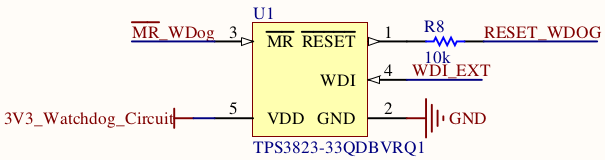
\includegraphics[width=0.65\textwidth]{figures/ext-watchdog-circuit.png}
        \caption{External watchdog timer circuit.}
        \label{fig:ext-wdt-circuit}
    \end{center}
\end{figure}

\section{Non-Volatile Memory}

The non-volatile memory model is the Micron MT25QL01GBBB, which is composed by a NOR flash architecture with 1 Gb of capacity (or 128 MB) and features extended SPI configurations. As can be seen in \autoref{fig:diagram-interfaces}, a SPI bus is used to communicate with this peripheral, using the \autoref{tab:usci-a0-config} configurations. Also, there are some control pins that are connected to microcontroller GPIOs: HOLD\#, RESET\#, and W\#. 

When RESET\# is driven LOW, the device is reset and the outputs are tri-stated. The HOLD\# signal pauses serial communications without deselecting or resetting the device, consequently outputs are tri-stated and inputs are ignored. The W\# signal handles as a write protection, which freezes the status register, turning its non-volatile bits read-only and preventing the write operation to be executed.


\begin{figure}[!ht]
    \begin{center}
        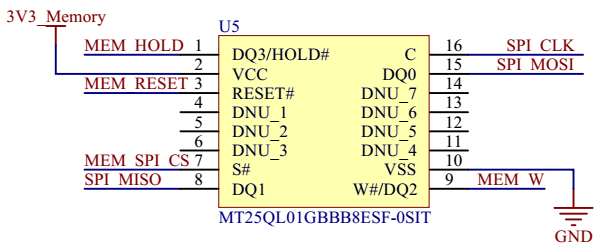
\includegraphics[width=0.65\textwidth]{figures/ext-memory-circuit.png}
        \caption{External memory circuit.}
        \label{fig:ext-mem-circuit}
    \end{center}
\end{figure}

\section{I2C Buffers}

The microcontroller I2C interfaces have dedicated IC buffers, which improve the signal quality throughout the various connectors and offers reliability enhancements, since it protects the bus in case of failures. This measure was adopted in all the satellite modules due to previous failures in I2C buses. Using this scheme, the modules connected though this protocol might have shared connections without losing performance or reliability. 

The buffer selected for this function is the Texas Instruments TCA4311 device. Besides the I2C inputs and outputs, it features control and status signals that are connected to GPIOs in the microcontroller: an enable and an operation ready status. Also, both inputs and outputs in these I2C lines have external pull-up resistors.

\begin{figure}[!ht]
    \begin{center}
        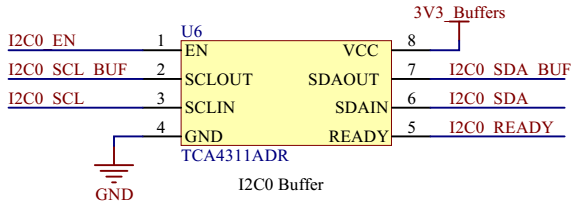
\includegraphics[width=0.65\textwidth]{figures/i2c-buffer-circuit.png}
        \caption{I2C buffer circuit.}
        \label{fig:i2c-buffer-circuit}
    \end{center}
\end{figure}

\section{RS-485 Transceiver}

The module features an RS-485 interface, which is connected to a 4H header (P8). This interface uses a transceiver (THVD1451) to convert the incoming RS-485 signals to UART and vice-versa. The outputs are 120 ohm differential pairs that have termination resistors before connecting to the header pins.

\begin{figure}[!ht]
    \begin{center}
        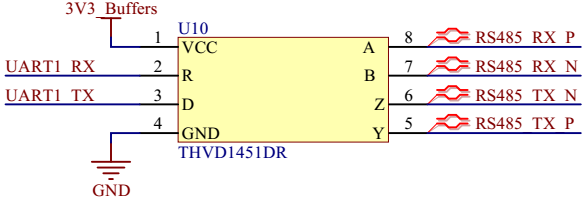
\includegraphics[width=0.65\textwidth]{figures/rs485-transceiver-circuit.png}
        \caption{RS-485 transceiver circuit.}
        \label{fig:rs485-transceiver-circuit}
    \end{center}
\end{figure}

\section{Voltage and Current Sensors}

In order to monitor the board overall current and voltage, the module have a current sensor using a Maxim Integrated IC (MAX9934) and a buffered voltage divider circuit with a Texas Instruments IC (TLV341A). These circuits have direct analog outputs that are connected to ADC inputs. The microcontroller internal ADC peripheral has a dedicated input for a voltage reference, which is connected to the REF5030A IC. This device generates a precise 3V output that enhances the measures and convertions performed by the microcontroller.

    %
% firmware.tex
%
% Copyright (C) 2019 by Universidade Federal de Santa Catarina.
%
% OBDH 2.0 Documentation
%
% This work is licensed under the Creative Commons Attribution-ShareAlike 4.0
% International License. To view a copy of this license,
% visit http://creativecommons.org/licenses/by-sa/4.0/.
%

%
% \brief Firmware chapter.
%
% \author Gabriel Mariano Marcelino <gabriel.mm8@gmail.com>
%
% \institution Universidade Federal de Santa Catarina (UFSC)
%
% \version 0.1.0
%
% \date 30/10/2019
%

\chapter{Firmware} \label{ch:firmware}

\section{Tasks}

A list of the firmware tasks can be seen in the \autoref{tab:firmware-tasks}.

\begin{table}[!h]
    \centering
    \begin{tabular}{lllll}
        \toprule[1.5pt]
        \textit{Name}          & \textit{Priority} & \textit{Initial delay [ms]} & \textit{Period [ms]} \\
        \midrule
        Startup (boot)         & Highest           & 0                           & Aperiodic            \\
        Deployment hibernation & Highest           & 0                           & Aperiodic            \\
        Antenna deployment     & Highest           & 0                           & Aperiodic            \\
        Watchdog reset         & Lowest            & 0                           & 100                  \\
        Heartbeat              & Lowest            & 0                           & 500                  \\
        Periodic downlink      & Medium            & 5000                        & 60000                \\
        Uplink                 & High              & 5000                        & 1000                 \\
        EPS reading            & Medium            & 5000                        & 60000                \\
        EDC reading            & High              & 5000                        & 1000                 \\
        Payload X reading      & Medium            & 5000                        & 5000                 \\
        TTC writing            & Medium            & 5000                        & Beacon period        \\
        Radio periodoc reset   & Low               & 0                           & 600000               \\
        OBDH reset             & Low               & 0                           & 36000000             \\
        \bottomrule[1.5pt]
    \end{tabular}
    \caption{Firmware tasks.}
    \label{tab:firmware-tasks}
\end{table}

All these tasks are better described below.

\subsection{Startup (boot)}

.

\subsection{Deployment hibernation}

.

\subsection{Antenna deployment}

.

\subsection{Watchdog reset}

.

\subsection{Heartbeat}

.

\subsection{Periodic downlink}

.

\subsection{Uplink}

.

\subsection{EPS reading}

.

\subsection{EDC reading}

.

\subsection{Payload X reading}

.

\subsection{TTC writing}

.

\subsection{Radio periodic reset}

.

\subsection{OBDH reset}

.

\section{Telecommands}

\begin{table}[!h]
    \centering
    \begin{tabular}{lll}
        \toprule[1.5pt]
        \textit{Name}          & \textit{Parameters}           & \textit{Access} \\
        \midrule
        Enter hibernation      & Hibernation period in seconds & Private         \\
        Leave hibernation      & None                          & Private         \\
        Activate beacon        & None                          & Private         \\
        Deactivate beacon      & None                          & Private         \\
        Activate downlink      & None                          & Private         \\
        Deactivate dtownlink   & None                          & Private         \\
        Activate EDC           & None                          & Private         \\
        Deactivate EDC         & None                          & Private         \\
        Activate Payload X     & Experiment period in seconds  & Private         \\
        Deactivate Payload X   & None                          & Private         \\
        Set system time        & Time value (epoch)            & Private         \\
        Ping                   & None                          & Public          \\
        Message broadcast      & ASCII message                 & Public          \\
        Request data           & Data flags                    & Public          \\
        \bottomrule[1.5pt]
    \end{tabular}
    \caption{System telecomamnds.}
    \label{tab:system-telecommands}
\end{table}

\section{Operating System}

FreeRTOS 10

\section{Hardware Abstraction Layer (HAL)}

DriverLib

\section{Protocols}

\subsection{NGHam}

NGHam \cite{ngham}, short for Next Generation Ham Radio, is a set of protocols for packet radio communication. Its usage is similar to the existing AX.25 protocol.

\begin{figure}[!ht]
    \begin{center}
        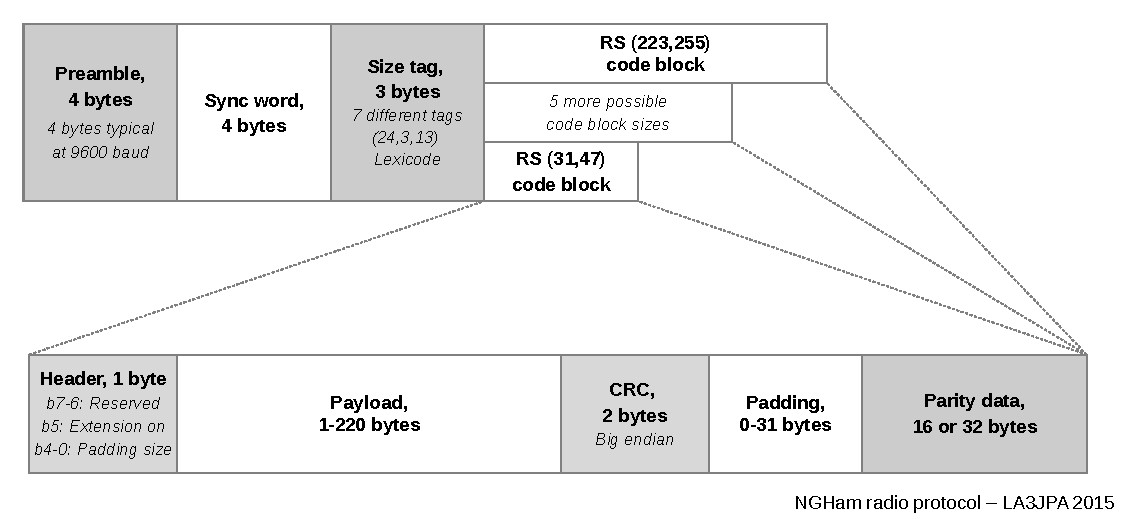
\includegraphics[width=\textwidth]{figures/ngham_block_v4.pdf}
        \caption{NGHam packet structure.}
        \label{fig:ngham-stack}
    \end{center}
\end{figure}

    %
% introduction.tex
%
% Copyright (C) 2020 by Universidade Federal de Santa Catarina.
%
% OBDH 2.0 Documentation
%
% This work is licensed under the Creative Commons Attribution-ShareAlike 4.0
% International License. To view a copy of this license,
% visit http://creativecommons.org/licenses/by-sa/4.0/.
%

%
% \brief References chapter.
%
% \author Gabriel Mariano Marcelino <gabriel.mm8@gmail.com>
%
% \institution Universidade Federal de Santa Catarina (UFSC)
%
% \version 0.5.0
%
% \date 2019/07/18
%

\bibliography{references/ngham,references/reliance_edge,references/msp430f6659,references/fsi-conn,references/tps382x,references/obdh2-repo}

\addcontentsline{toc}{chapter}{References}


\end{document}
